    
		 \section{TI nspire CX CAS}
		 \begin{tabular}{ll}
		 \textbf{Zweck} & \textbf{Befehl} \\
		 Matrix erstellen & menu - 7 - 1 \\ 
		 Skalarprodukt & dotP([Vektor], [Vektor])\\
		 Kreuzprodukt  & crossP([Vektor], [Vektor])\\
		 Gauss-Algorithmus RREF & menu - 7 - 5\\
		 Zeilenoperationen & menu - 7 - 9 - X \\
		 Determinante & menu - 7- 3\\
		 Matrix transponieren &  menu - 7- 2\\
		 Matrix invertieren & $[\text{Matrix}]^{-1}$ \\
		 Spur & menu - 7 - B - 1 \\
		 LR-Zerlegung & menu - 7 - B - 2 \\
		 QR-Zerlegung & menu - 7 - B - 3 \\
		 Eigenwerte & menu - 7 - B - 4 \\
		 Eigenvektoren & menu - 7 - B - 5 \\
		 Char. Polynom & menu - 7 - B - 6 \quad charPoly(Matrix, x) 
		 \end{tabular}
		    
		    
		    
		    
		    
		 \section{Anwendungsbeispiele aus der Vorlesung}
		 %hier sind bewusst nur die Folien aus den Vorlesungen eingefügt, damit auf der ausgedrucken Form der Zusammenfassung individuelle Notizen gemacht werden können
		 
		 \subsection{Matrixoptik}
		 
		 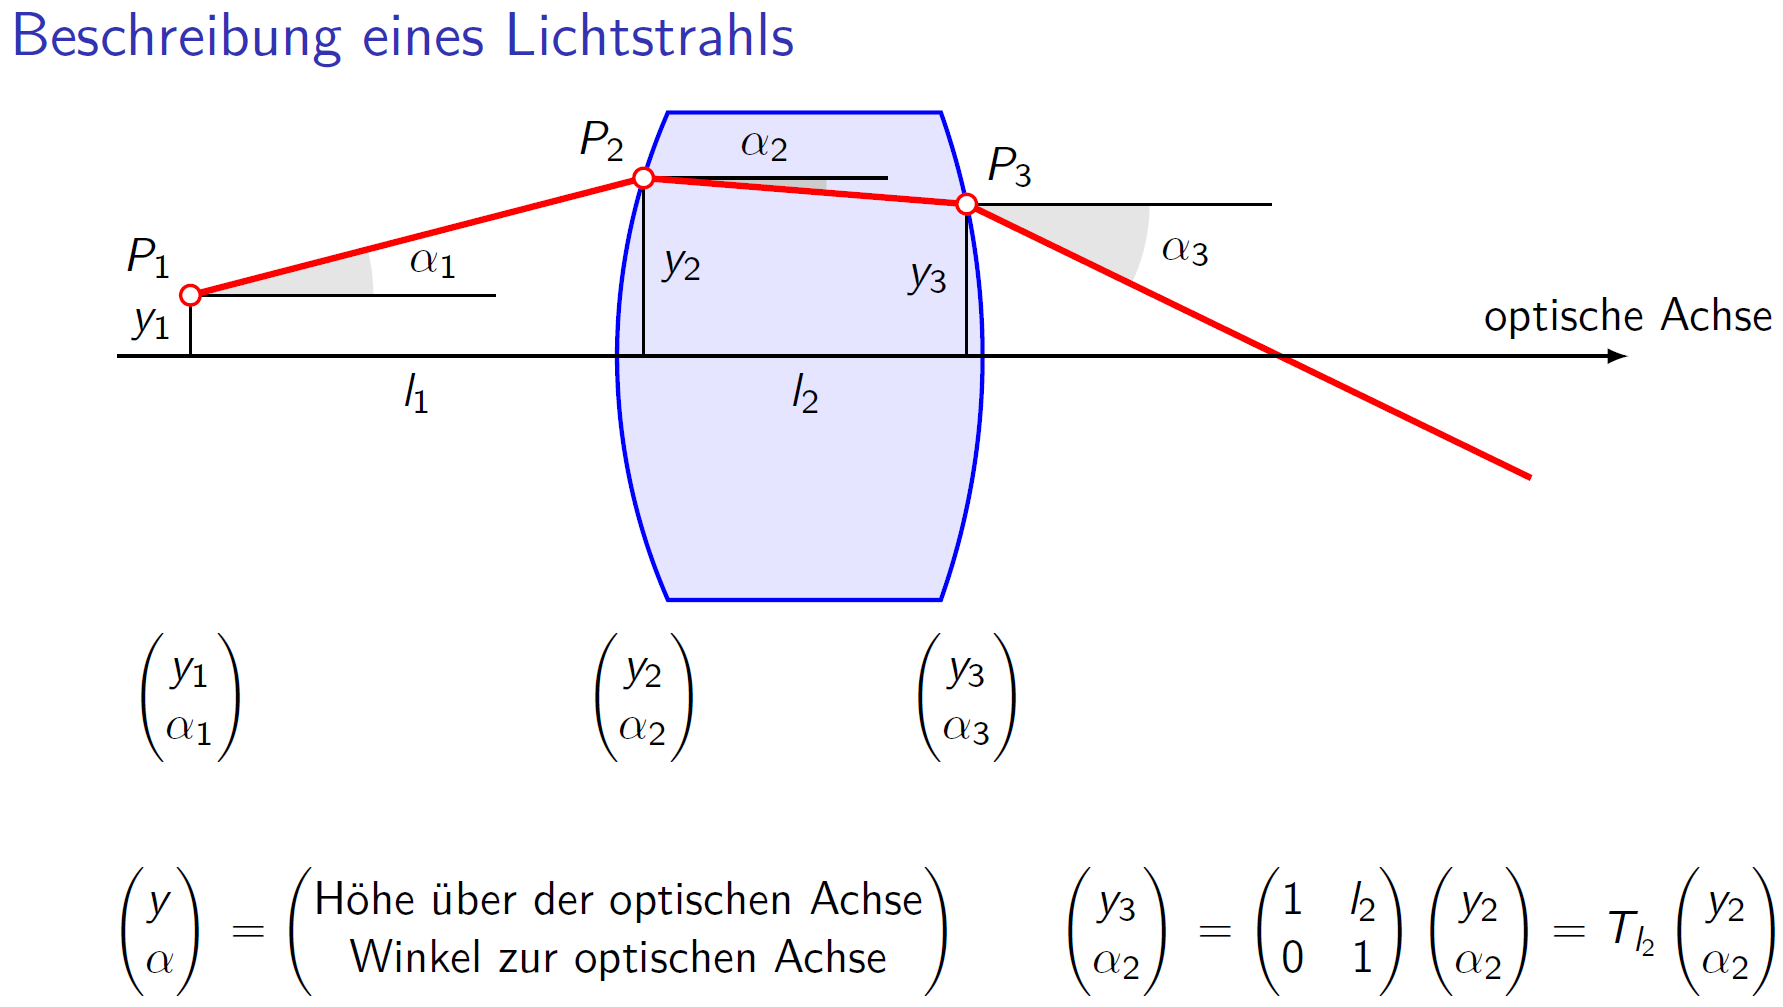
\includegraphics[width=0.85\linewidth]{Bilder/matrixoptik1} \\
		 
		 \vspace{0.5cm}
		 
		 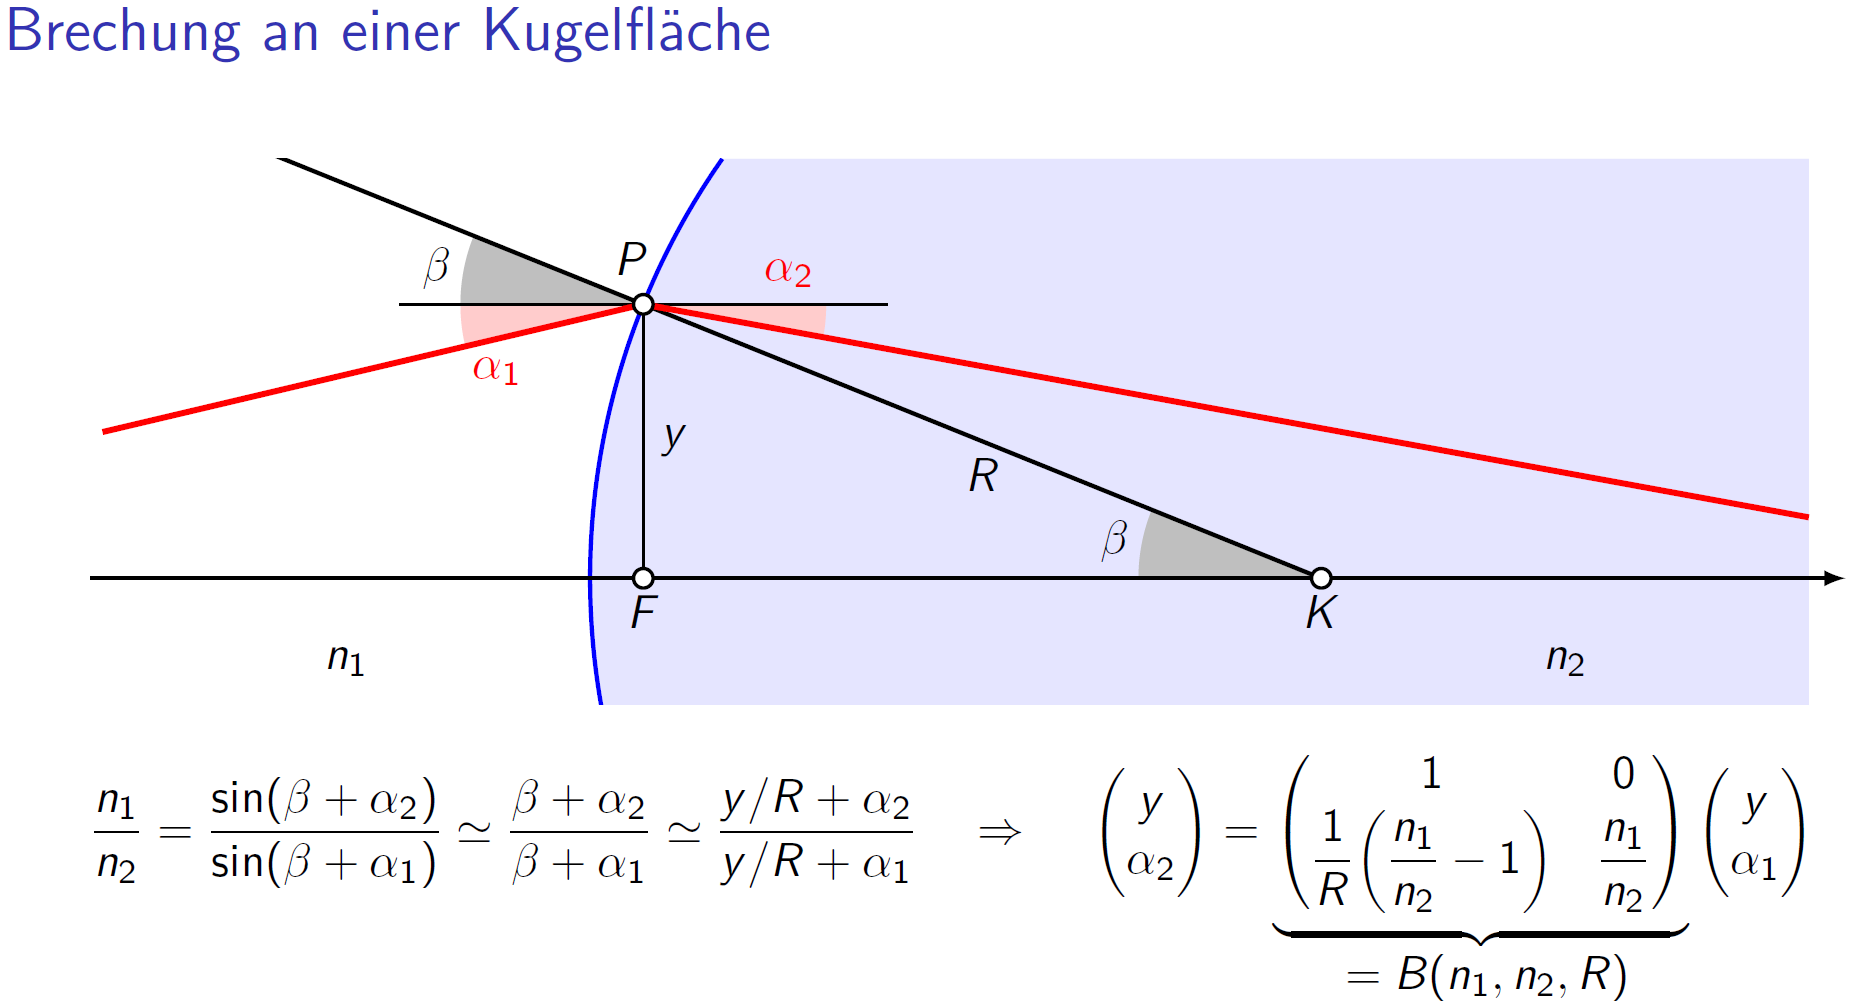
\includegraphics[width=0.85\linewidth]{Bilder/matrixoptik2} \\
		 
		 \vfill\null
		 \columnbreak
		 
		 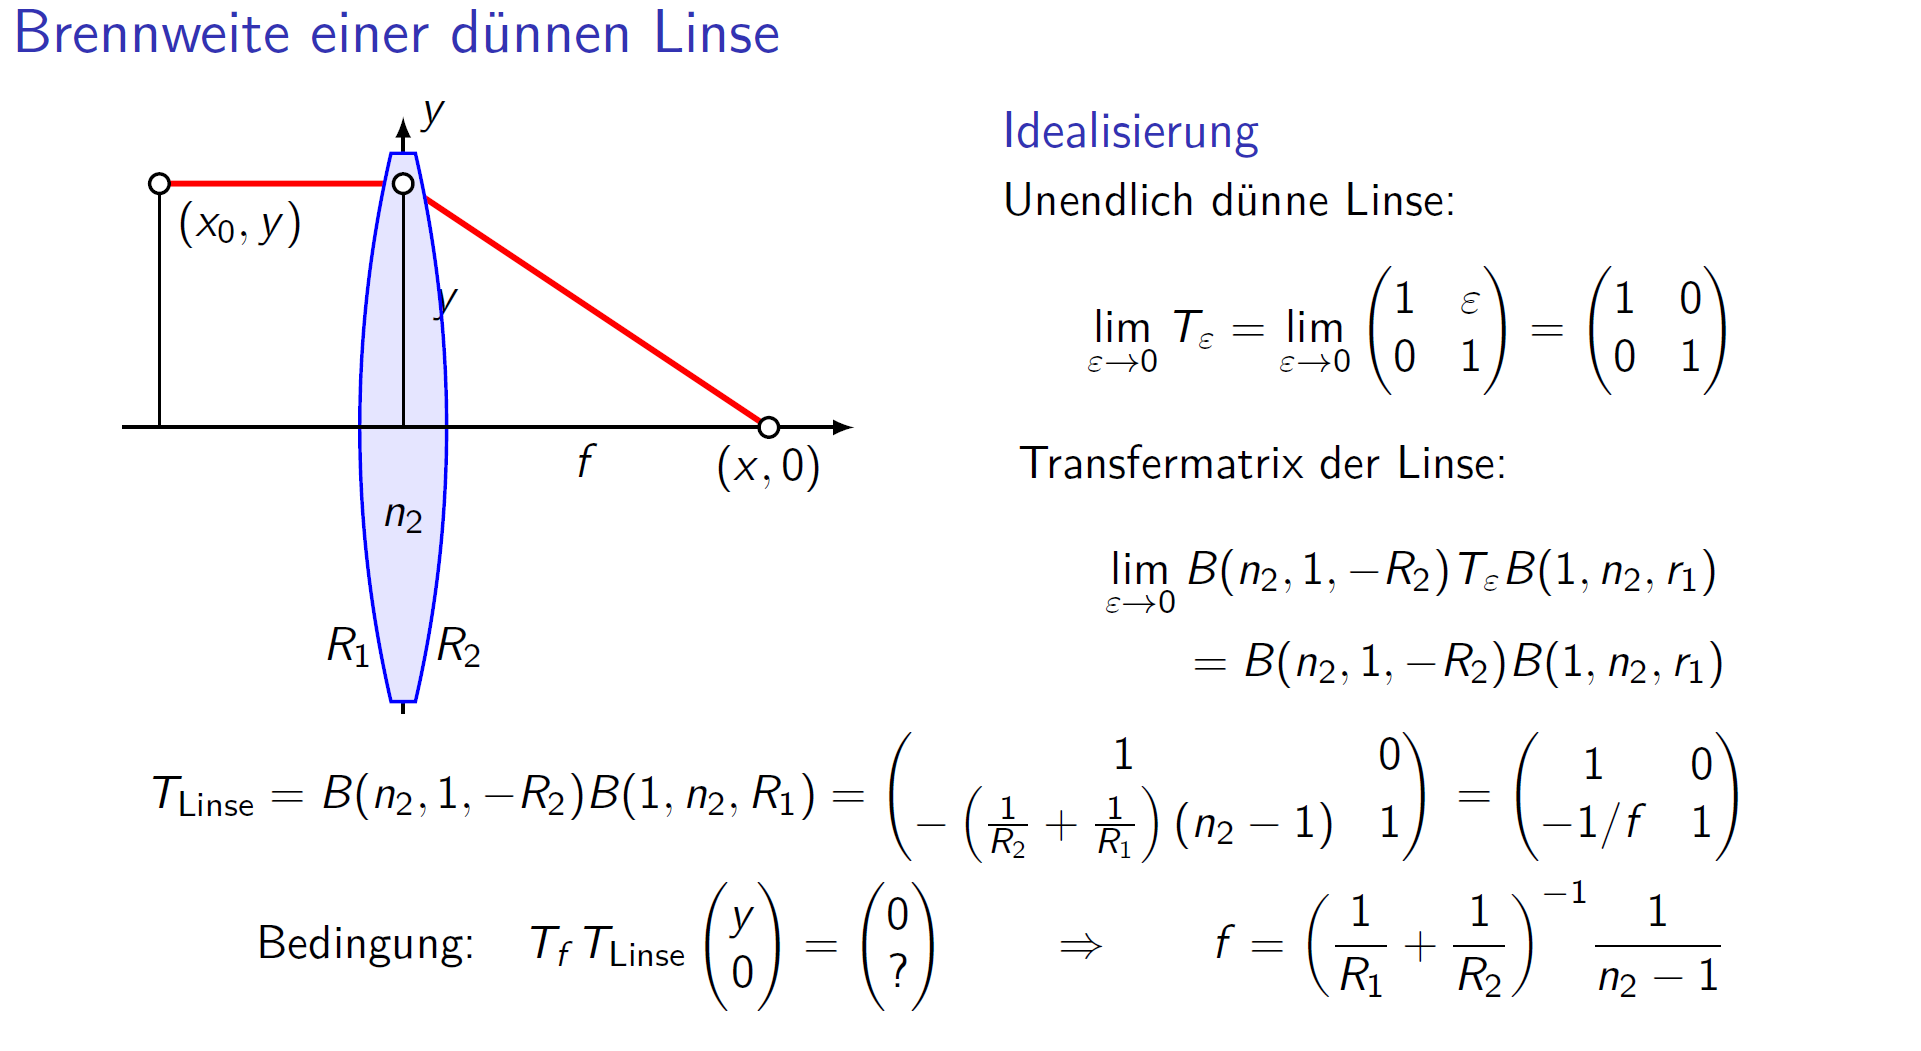
\includegraphics[width=0.8\linewidth]{Bilder/matrixoptik3} \\
		 
		 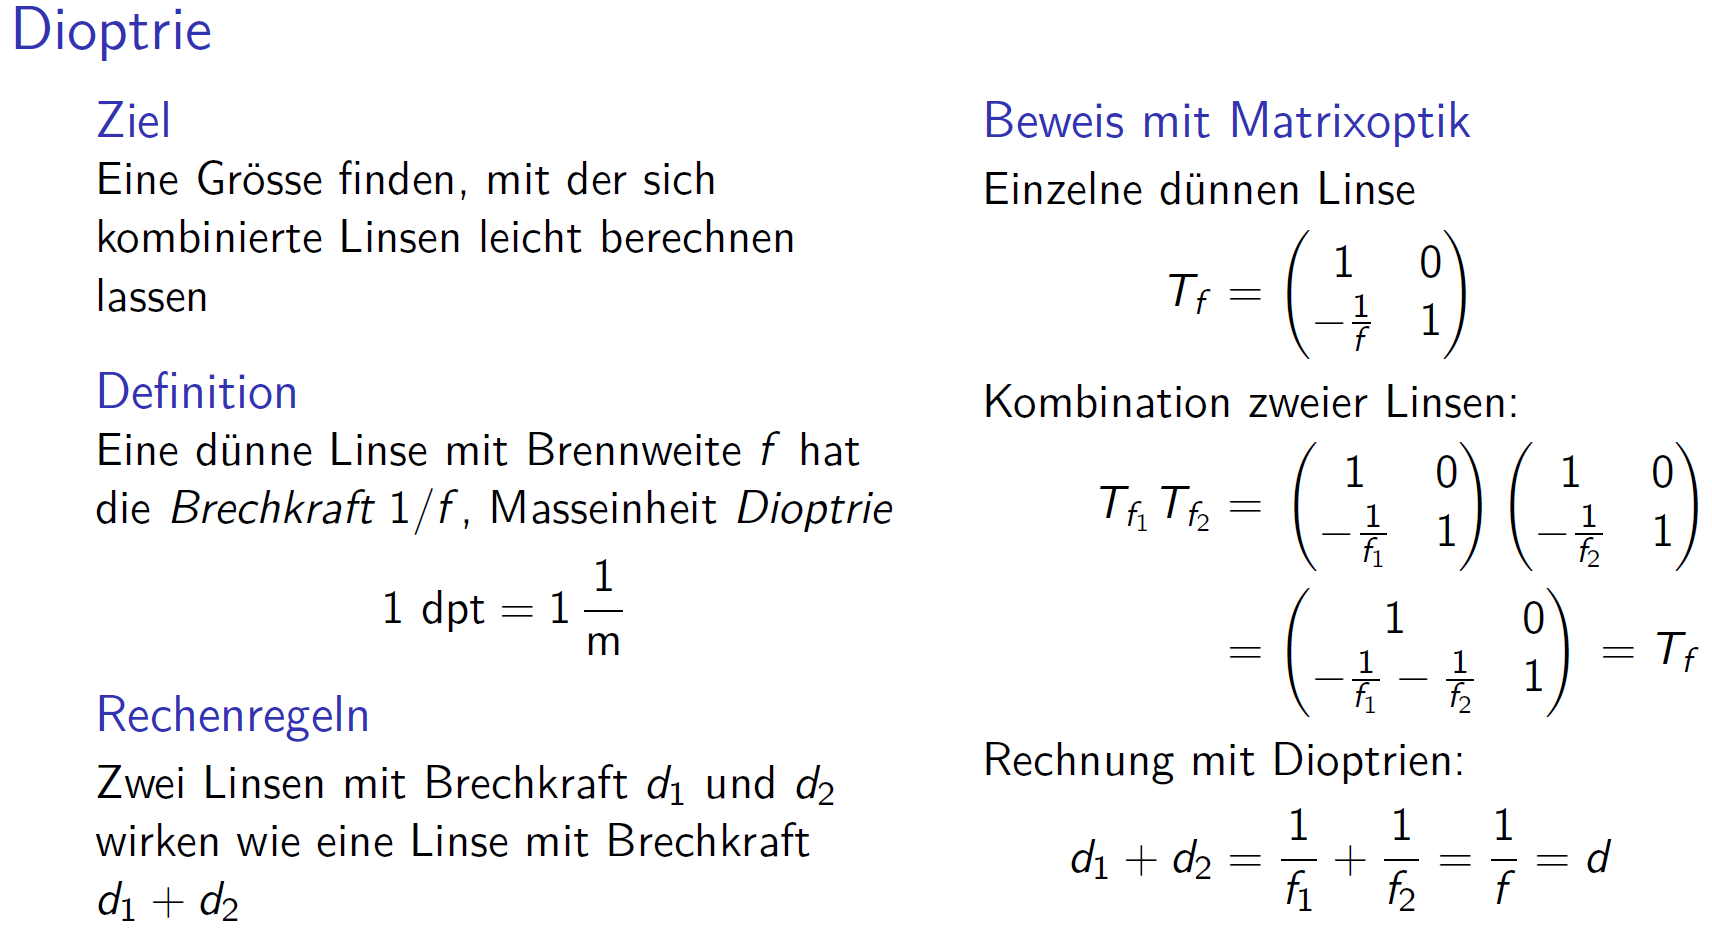
\includegraphics[width=0.8\linewidth]{Bilder/matrixoptik4} \\
		 
		 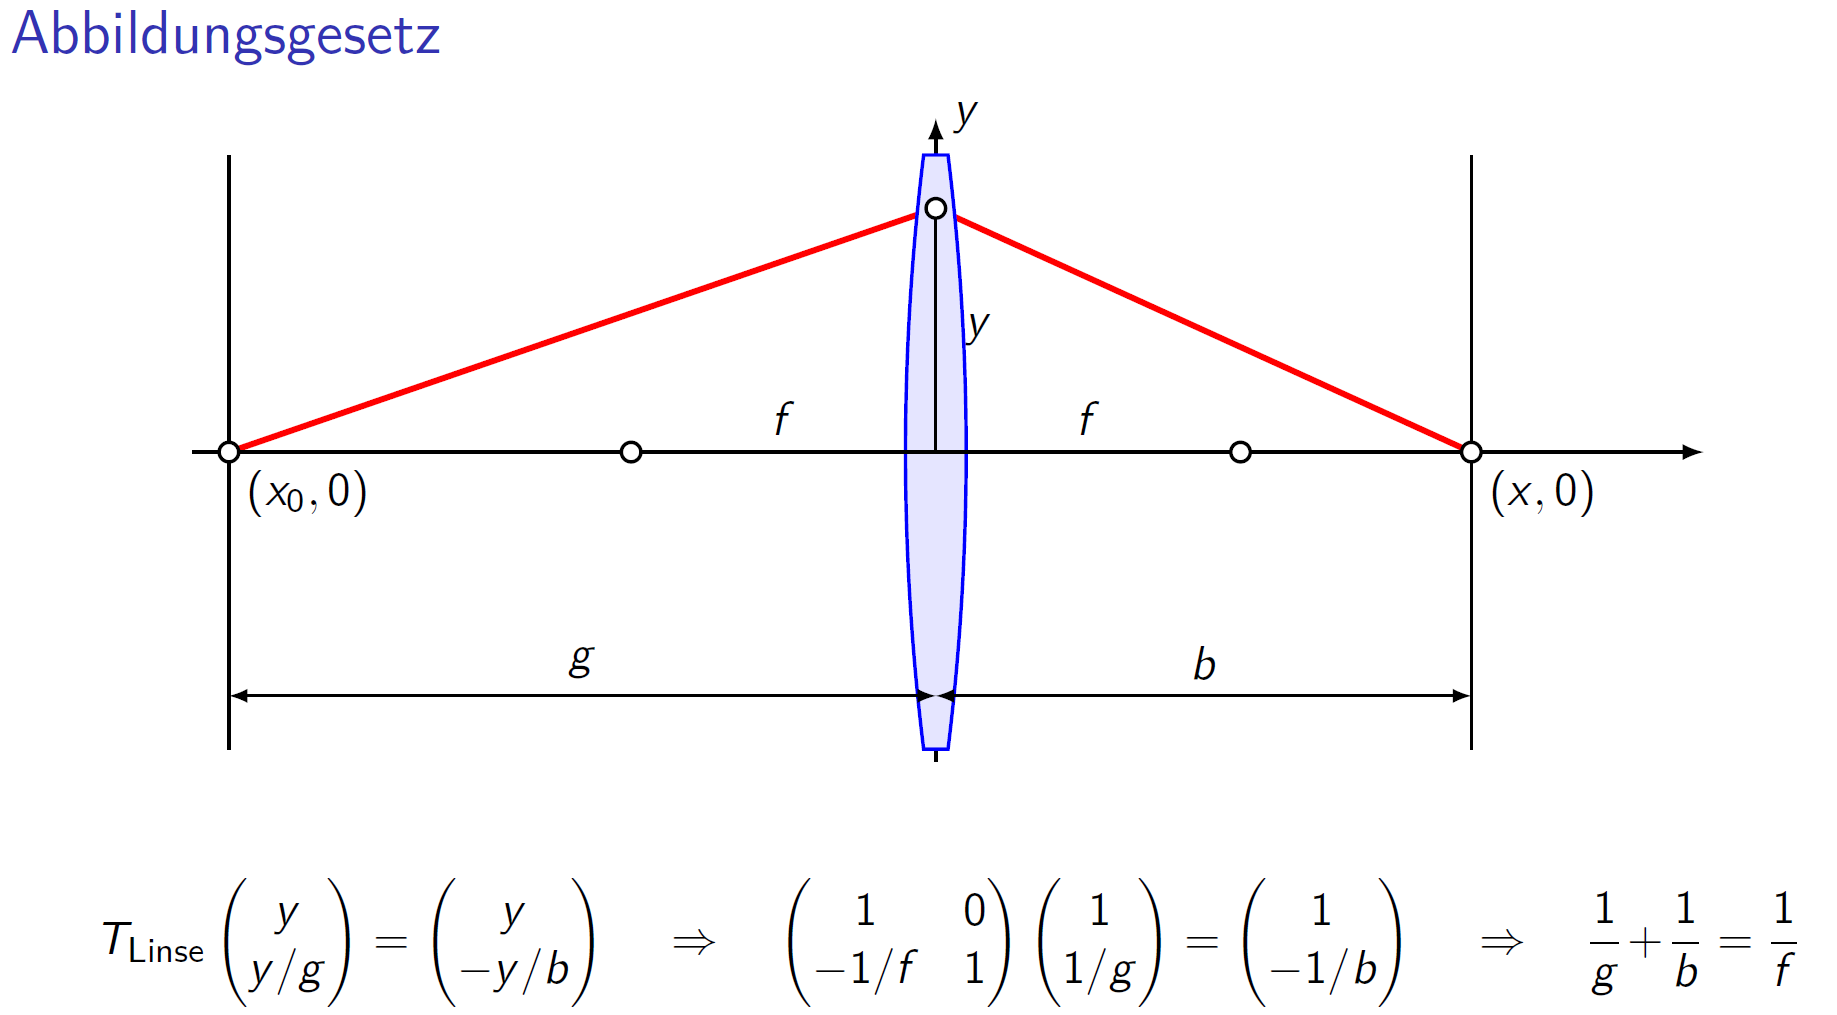
\includegraphics[width=0.8\linewidth]{Bilder/matrixoptik5}\\
		 
		 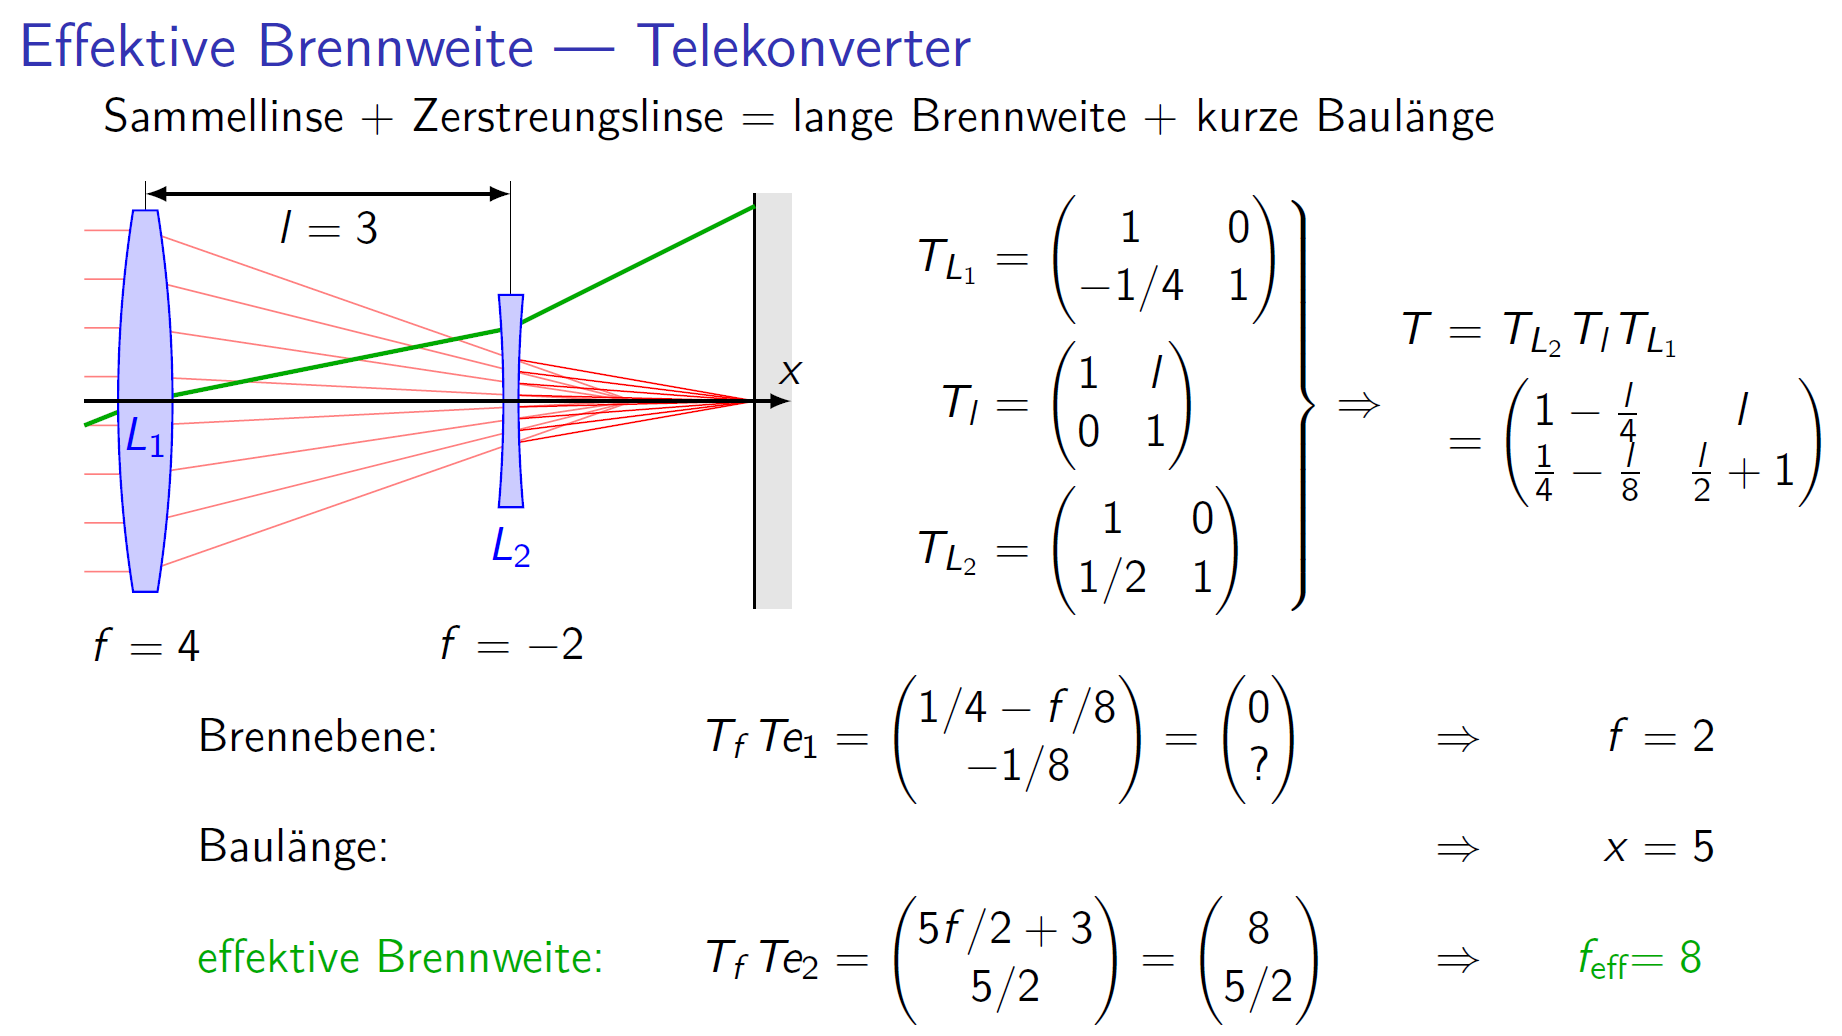
\includegraphics[width=0.8\linewidth]{Bilder/matrixoptik6} \\
		
		 
		 
		 \subsection{Kettenbrüche}
		 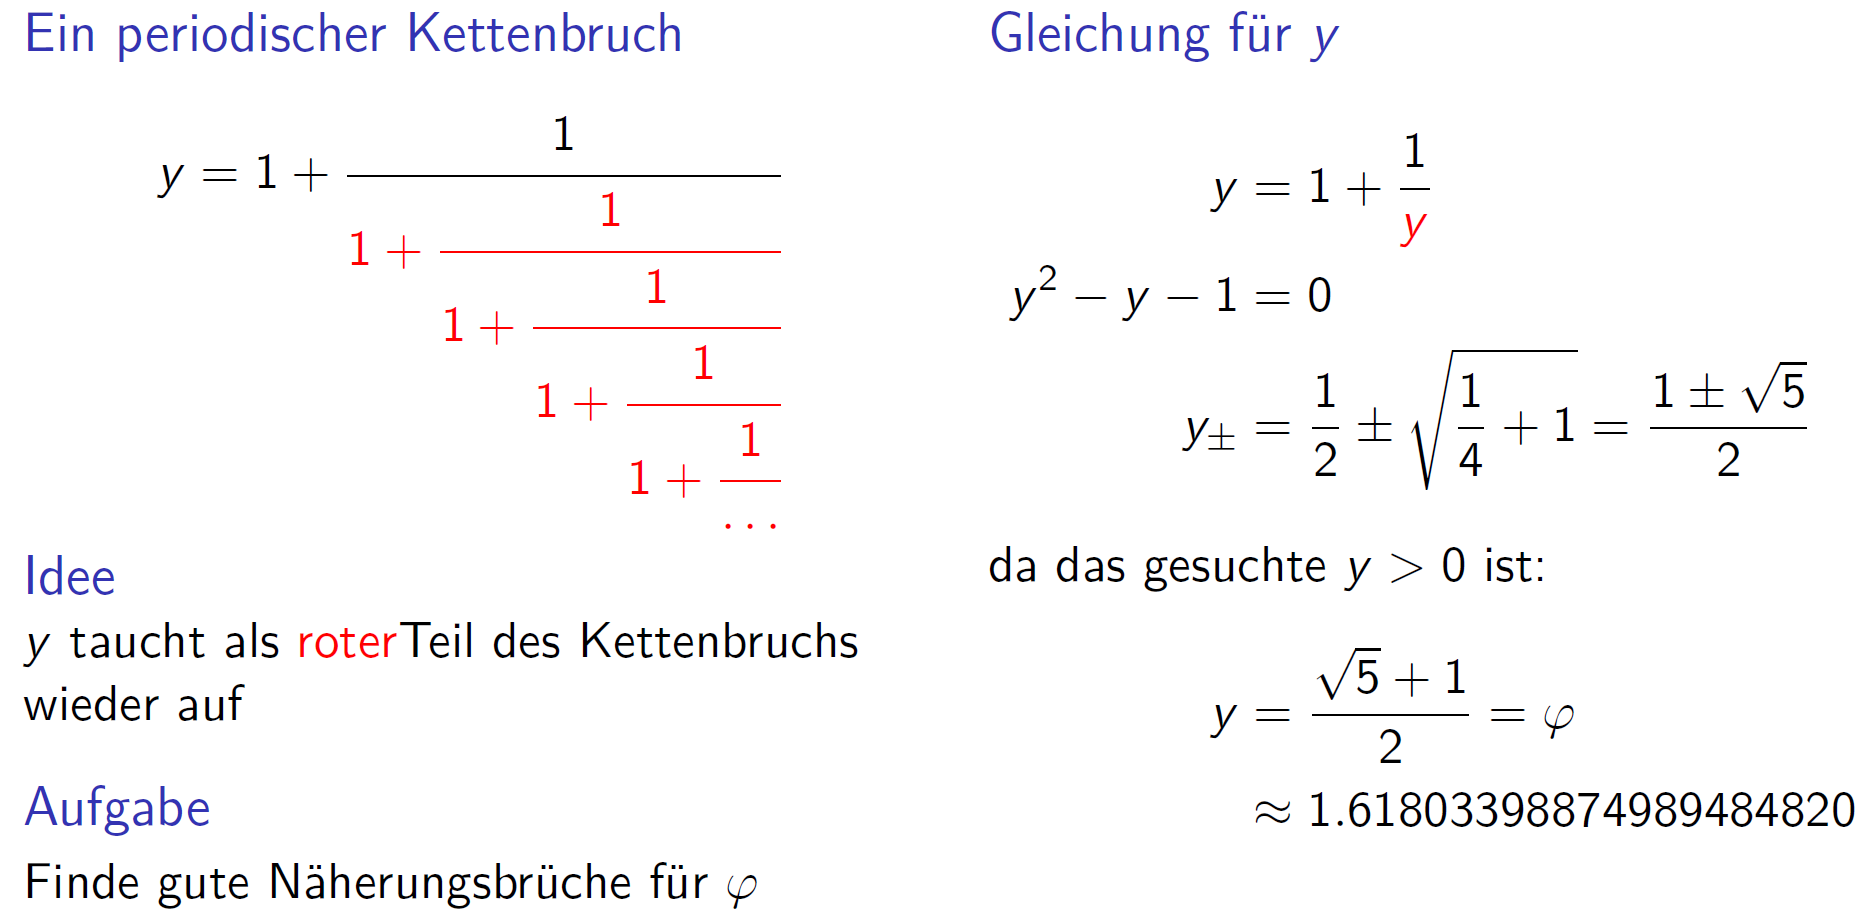
\includegraphics[width=0.8\linewidth]{Bilder/kettenbruch1} \\
		 
		 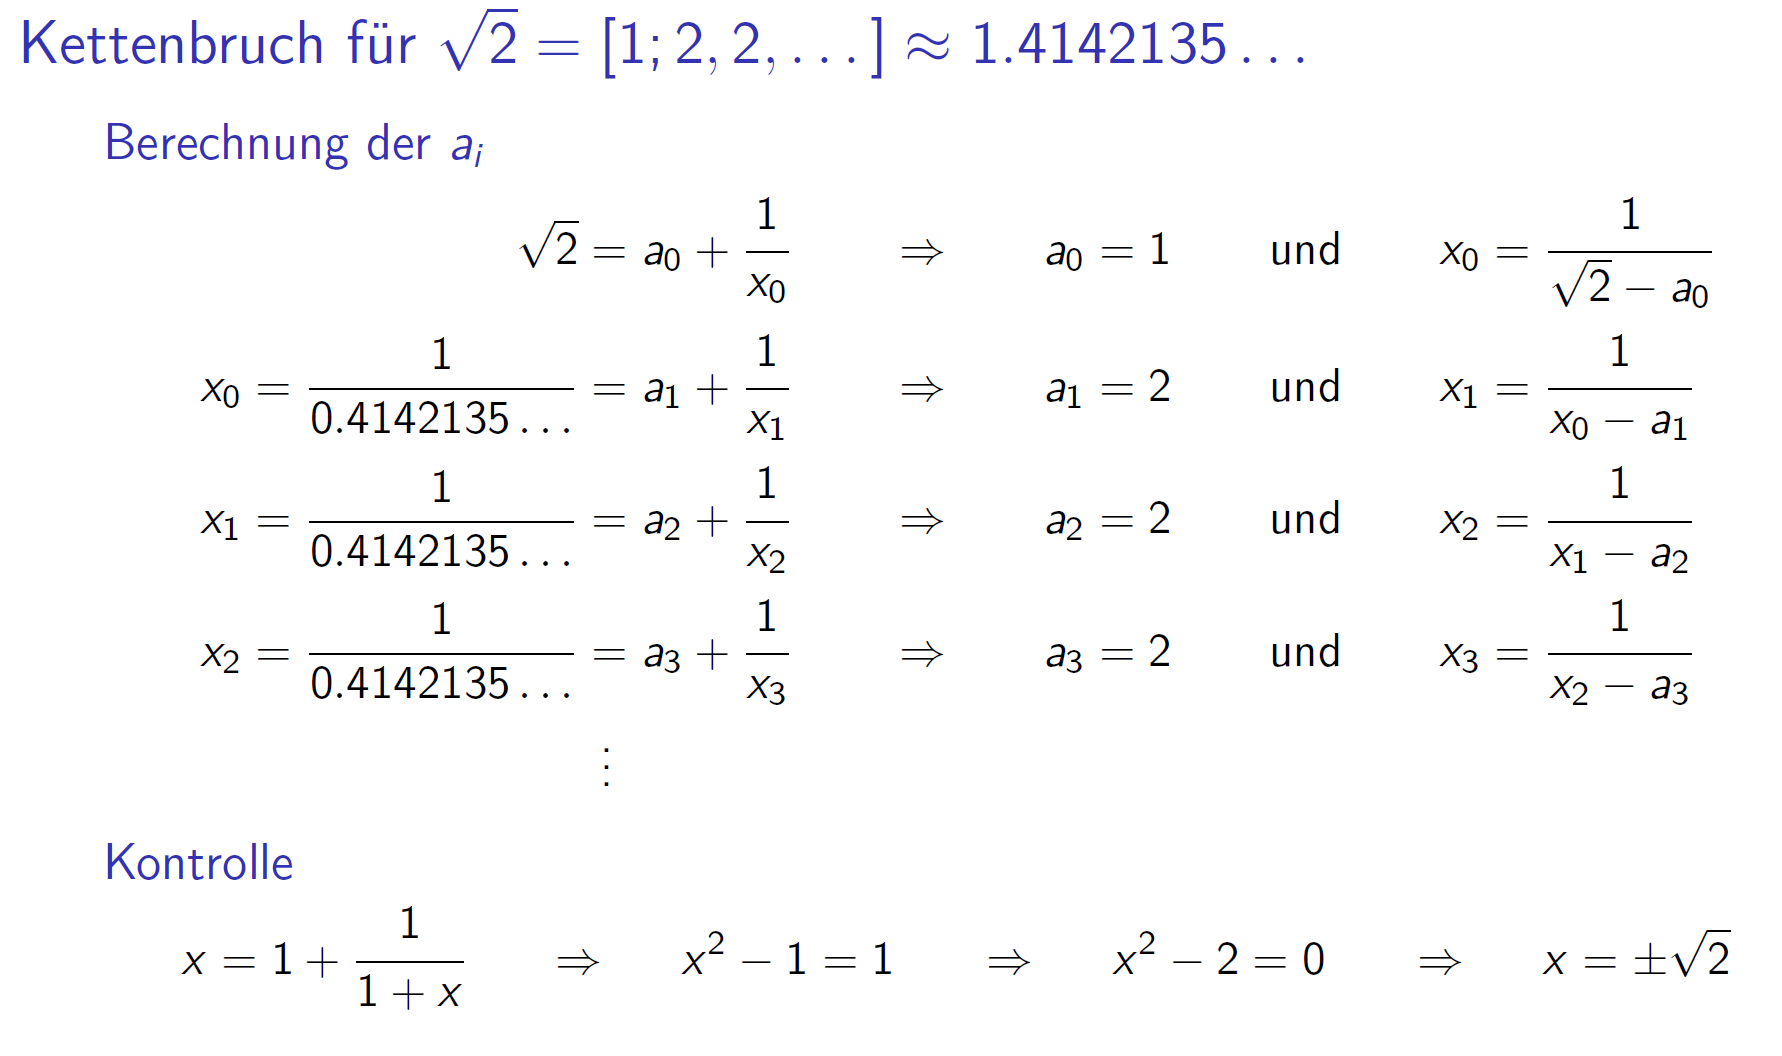
\includegraphics[width=0.8\linewidth]{Bilder/kettenbruch2} \\
		 
		 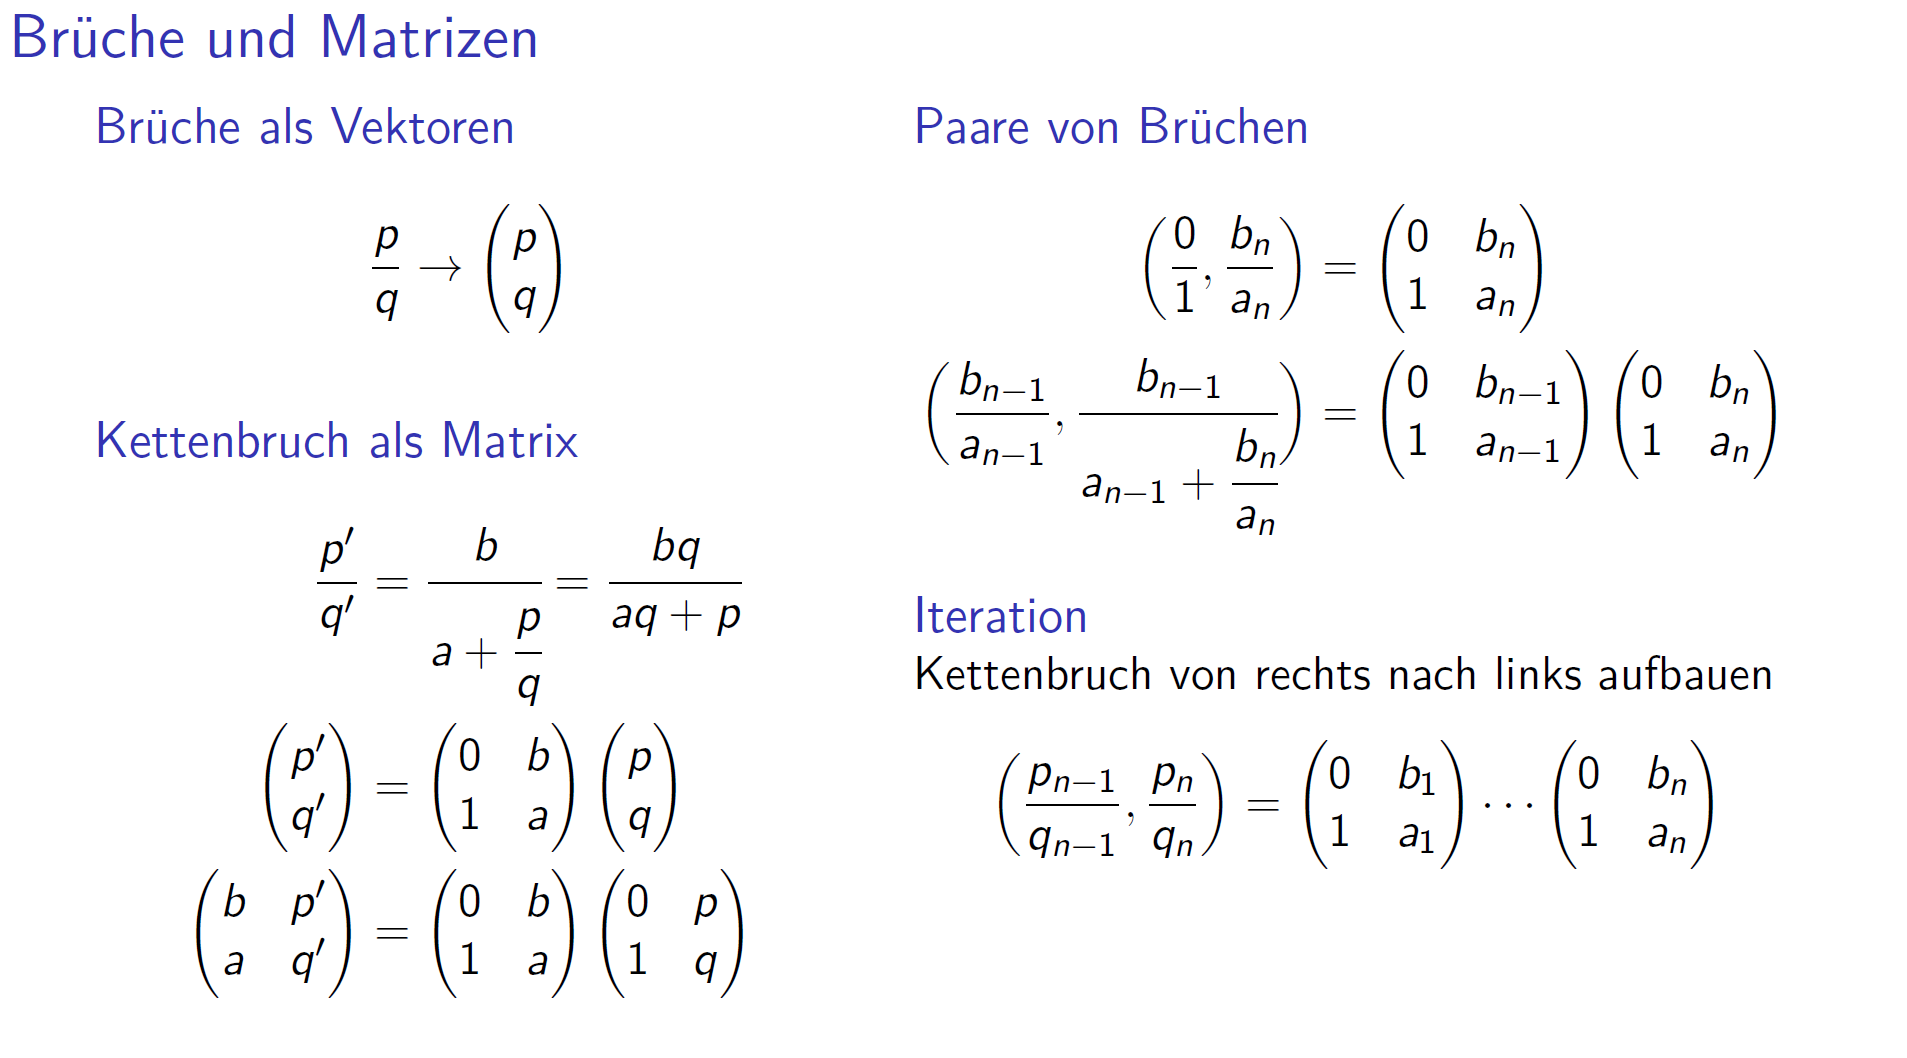
\includegraphics[width=0.8\linewidth]{Bilder/kettenbruch3} \\
		 
		 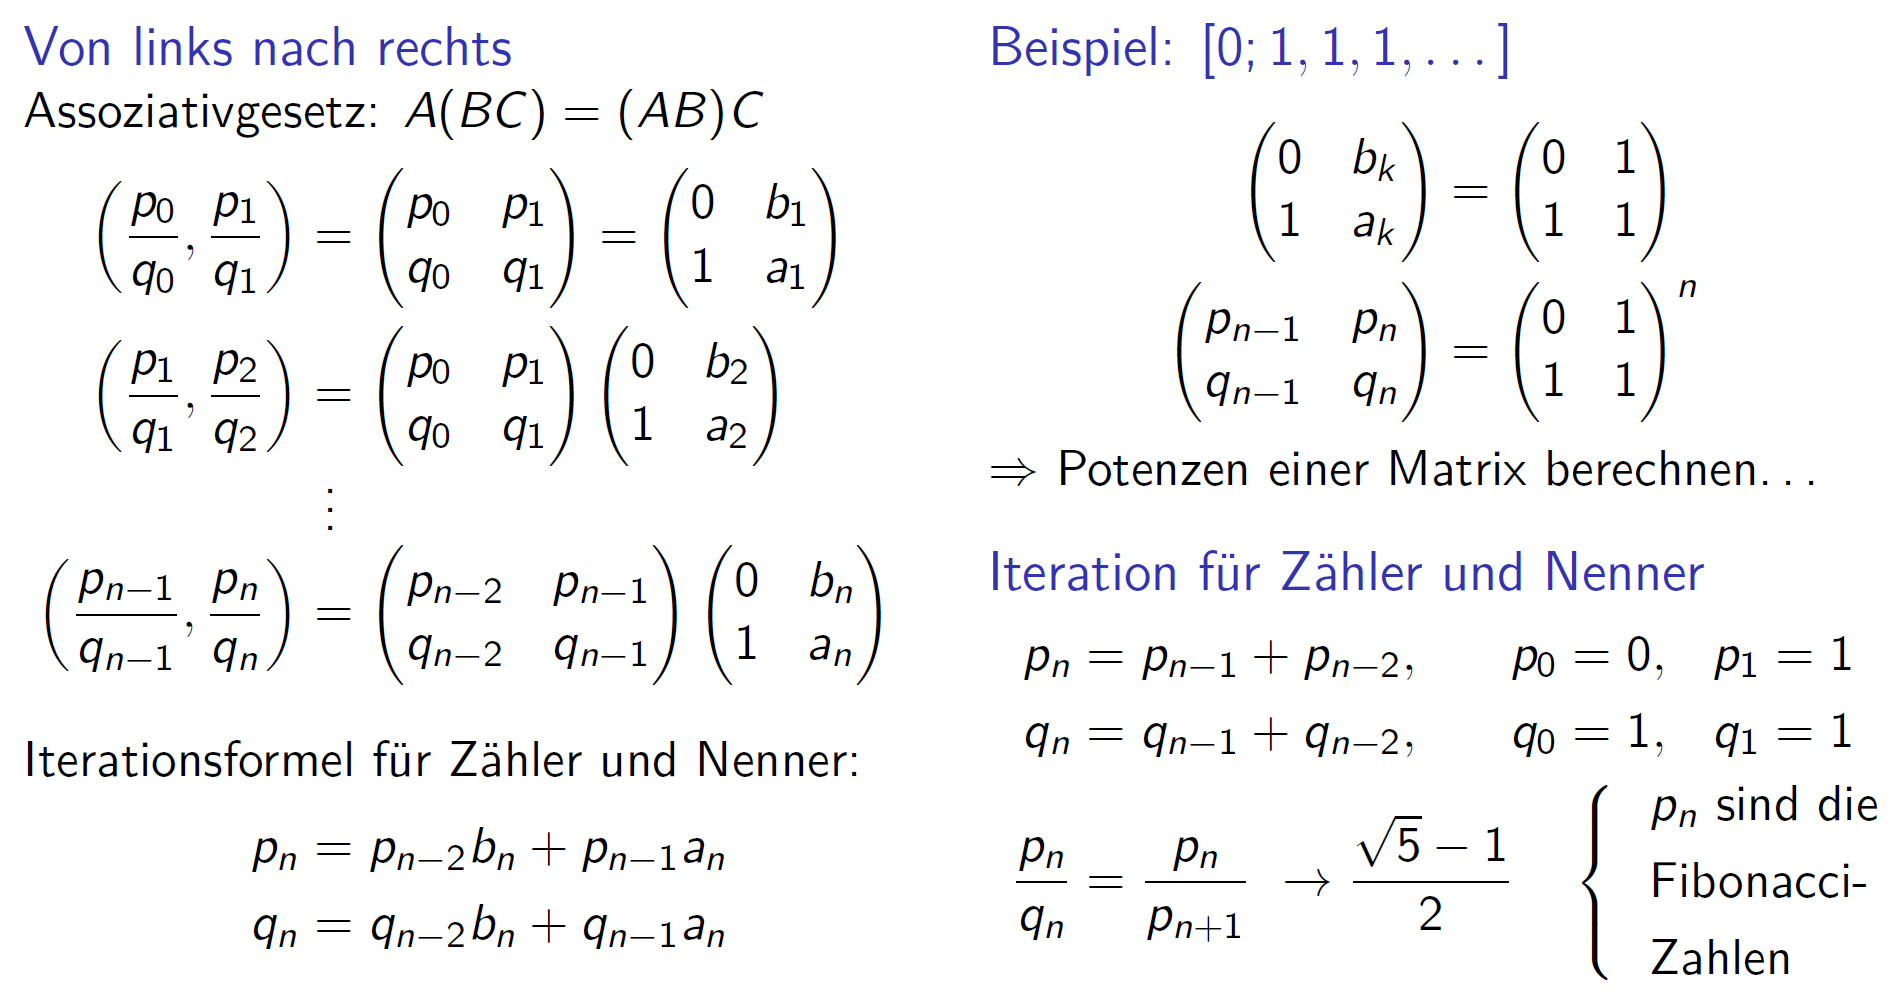
\includegraphics[width=0.8\linewidth]{Bilder/kettenbruch4} \\
		 
		 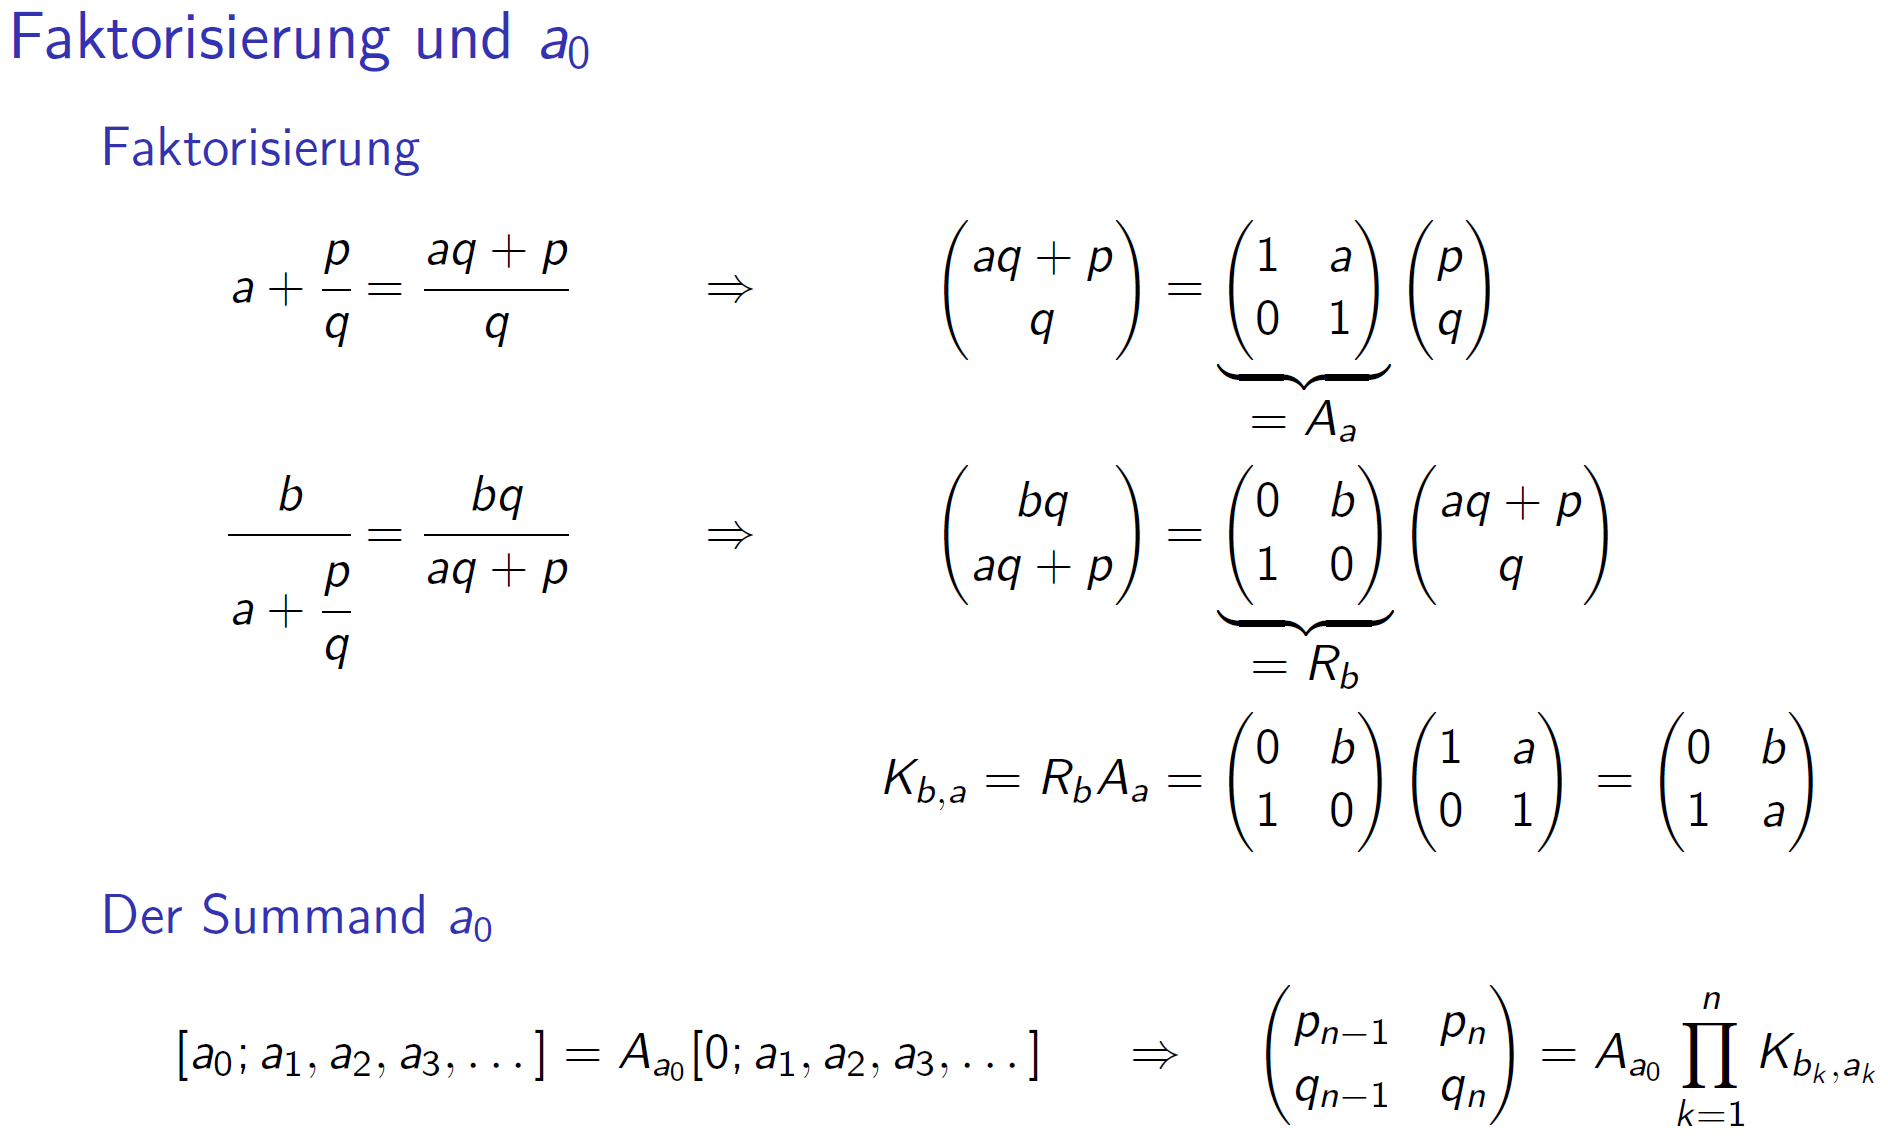
\includegraphics[width=0.8\linewidth]{Bilder/kettenbruch5} \\
		  
		 
		 
		 
		 \subsection{Rekursionsformeln}
		 \textbf{Anwendung Eigenwerte / Eigenvektoren / Eigenbasis} \\
		 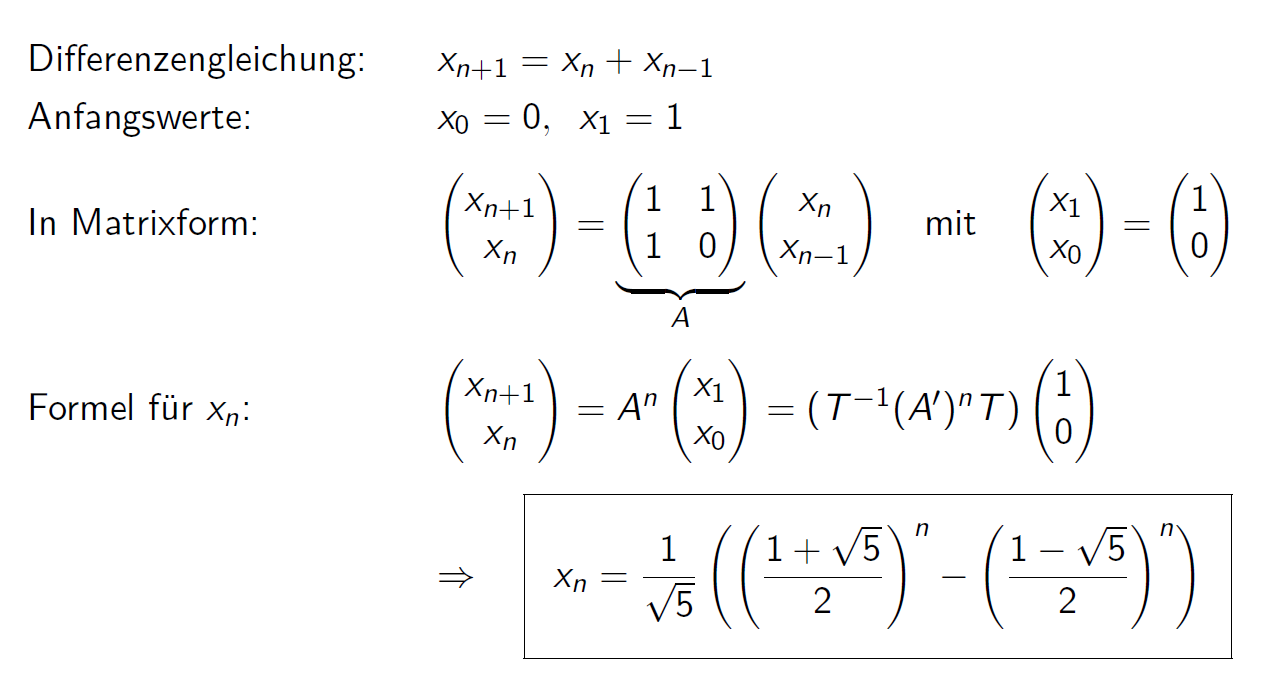
\includegraphics[width=0.8\linewidth]{Bilder/rekursion1} \\ 
		 
		 
		 
		 
		\subsection{Kamerageometrie}		 
		 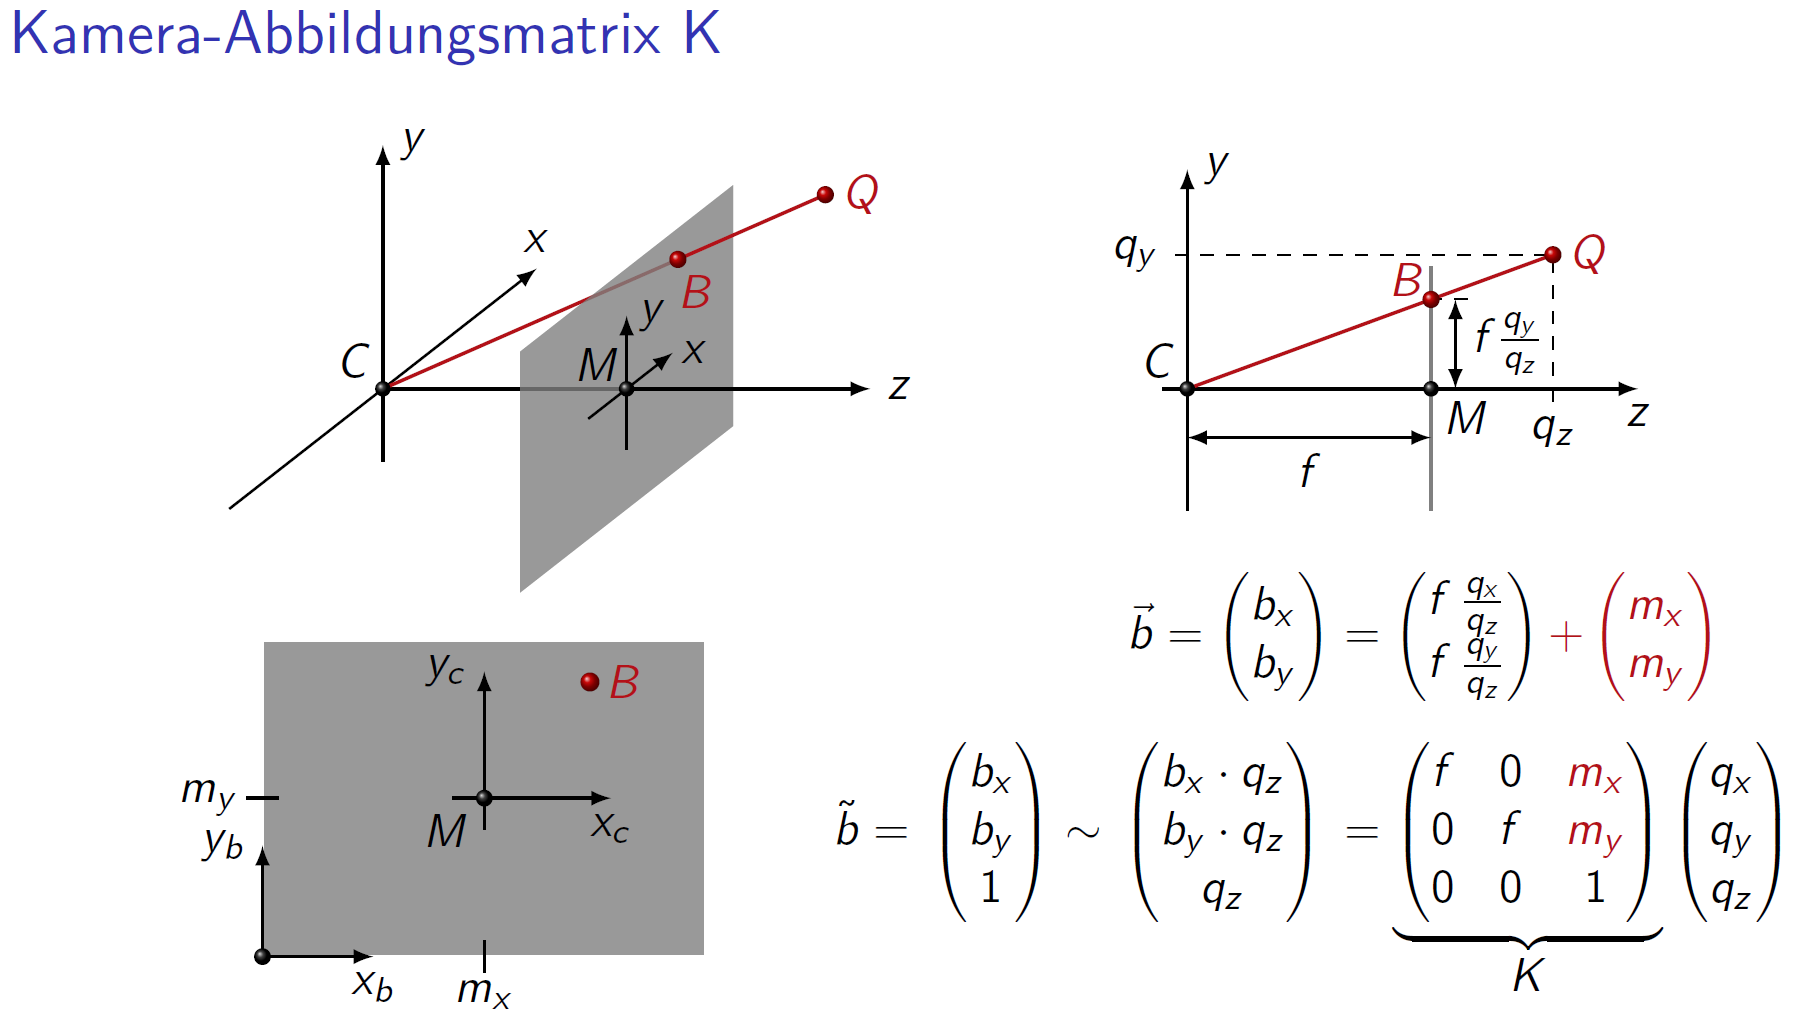
\includegraphics[width=0.9\linewidth]{Bilder/kamera1} \\
		 
		 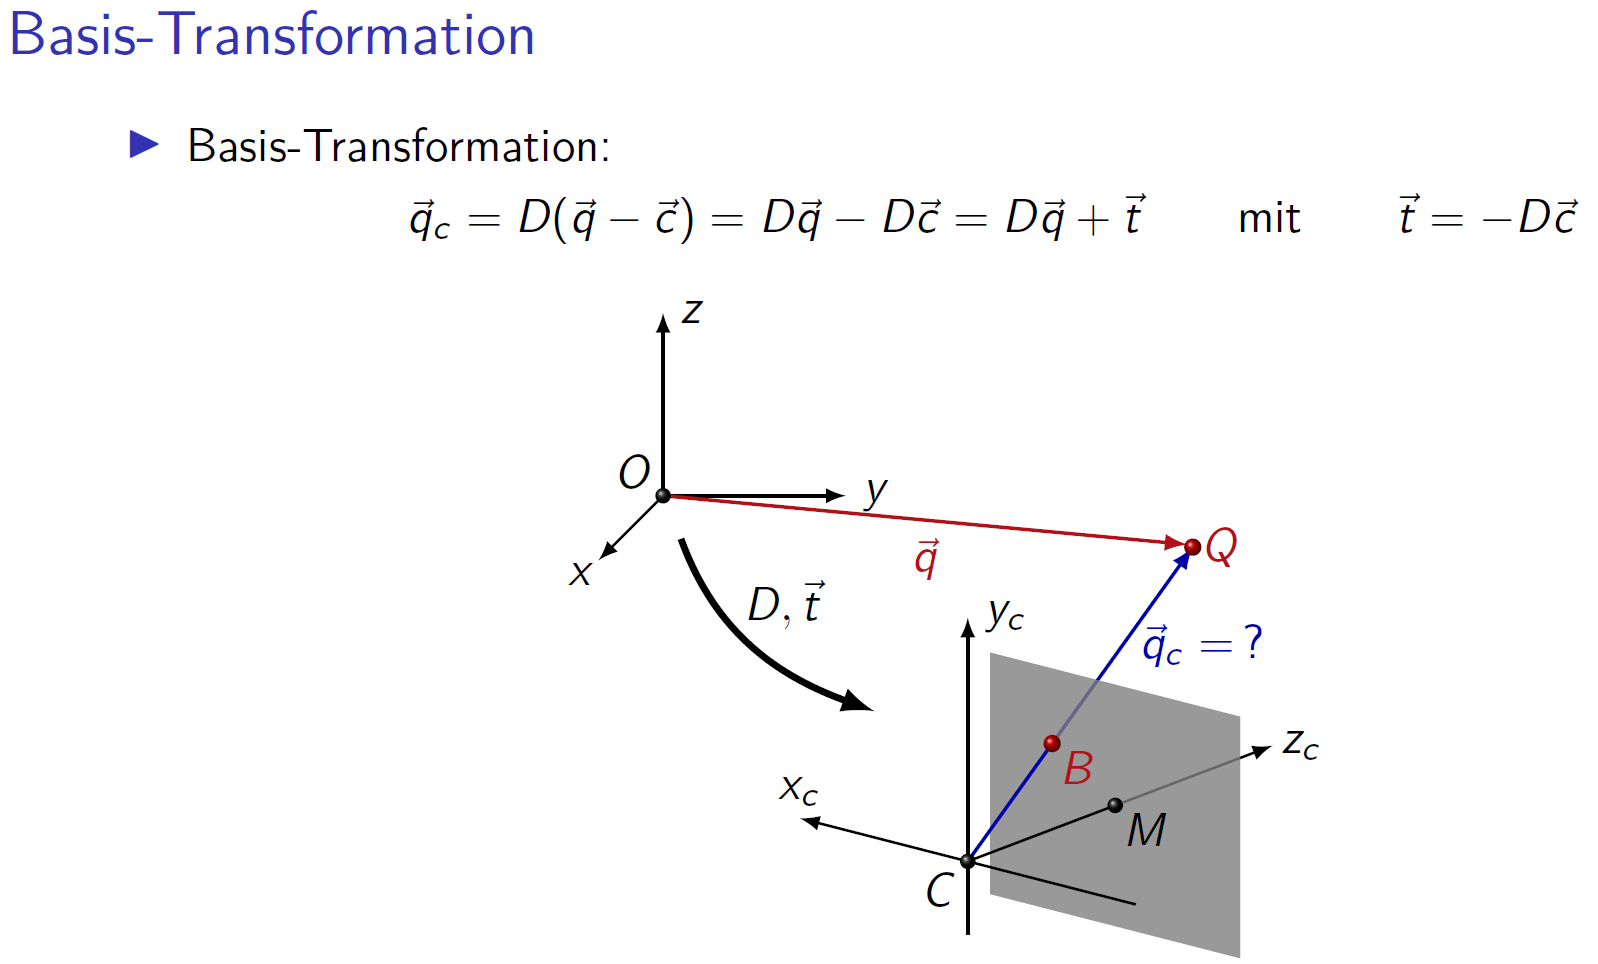
\includegraphics[width=0.9\linewidth]{Bilder/kamera2} \\
		 
		 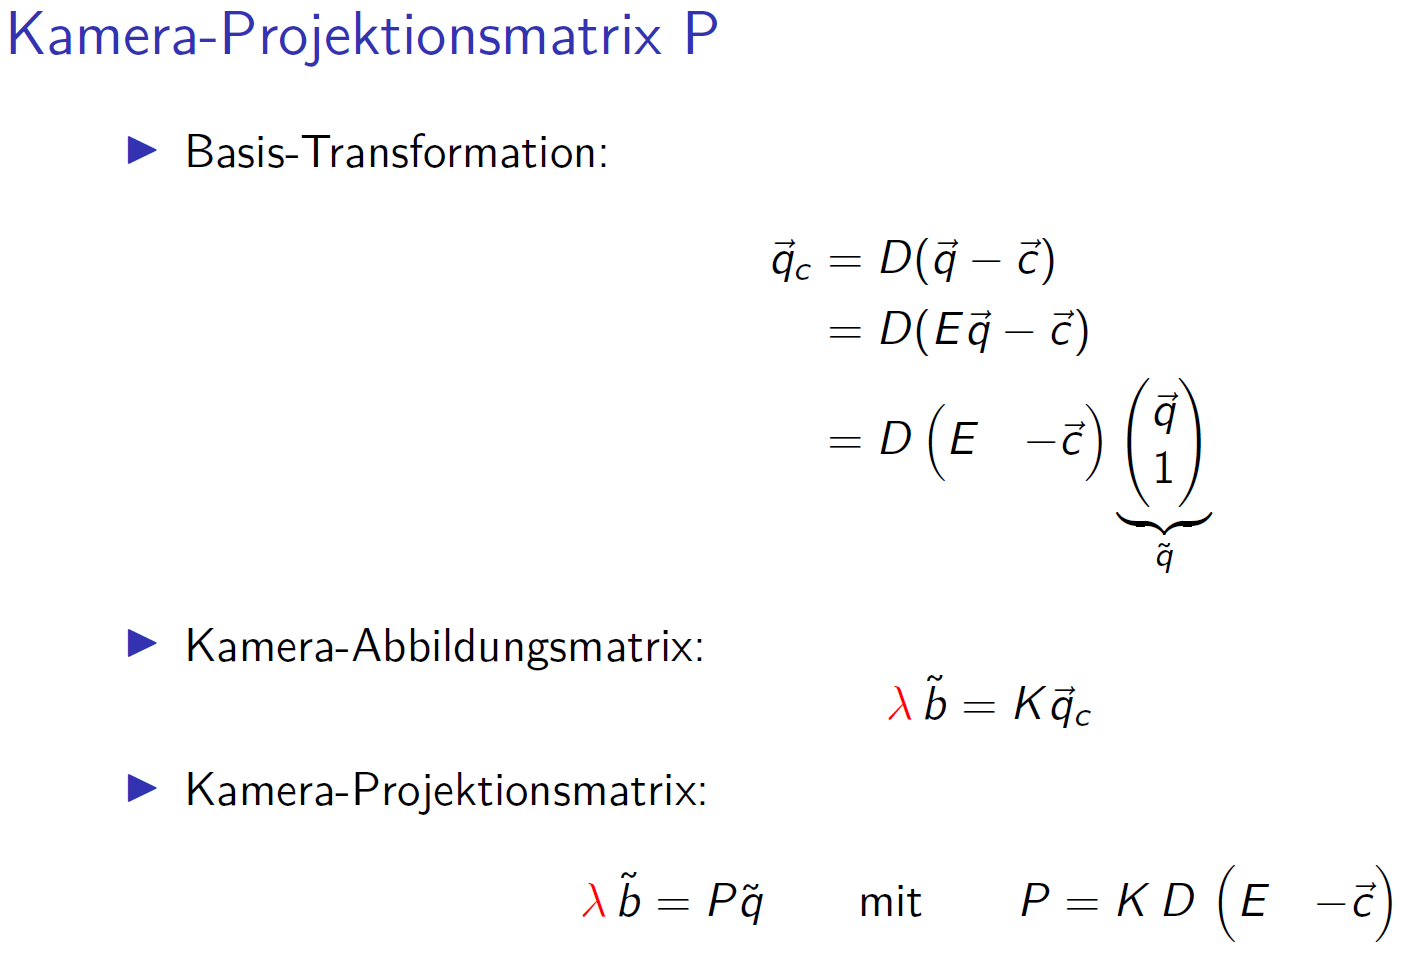
\includegraphics[width=0.9\linewidth]{Bilder/kamera3} \\
		 
		 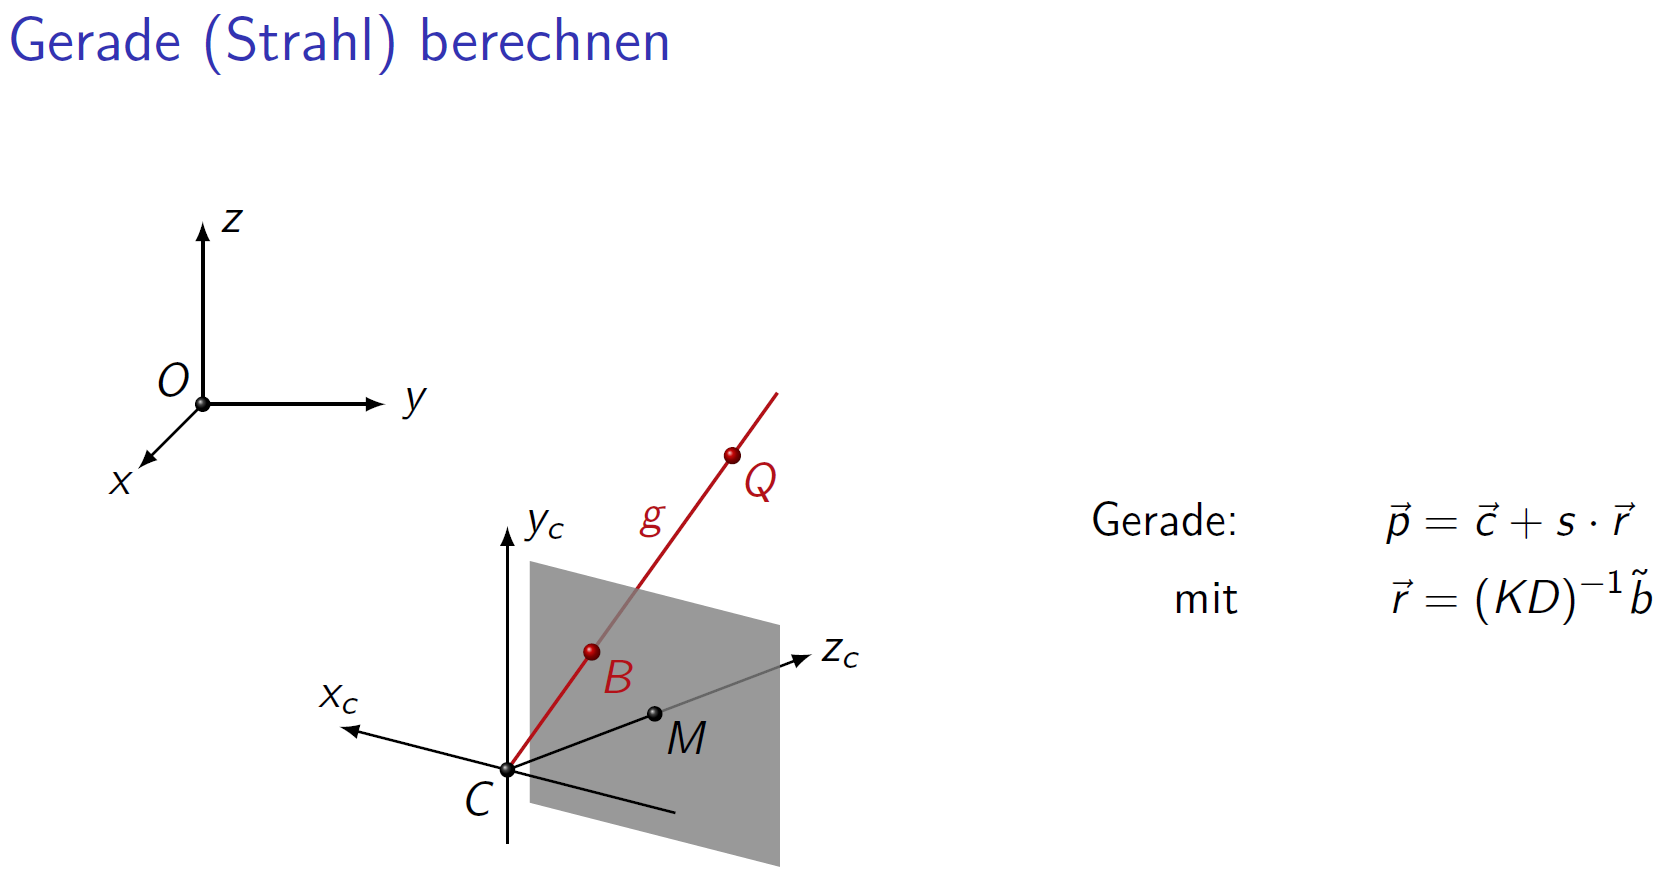
\includegraphics[width=0.9\linewidth]{Bilder/kamera4} 	 
		 
		 
		 
		 
		 
		       
		    
		
		  \subsection{Widerstandsnetzwerk}
		   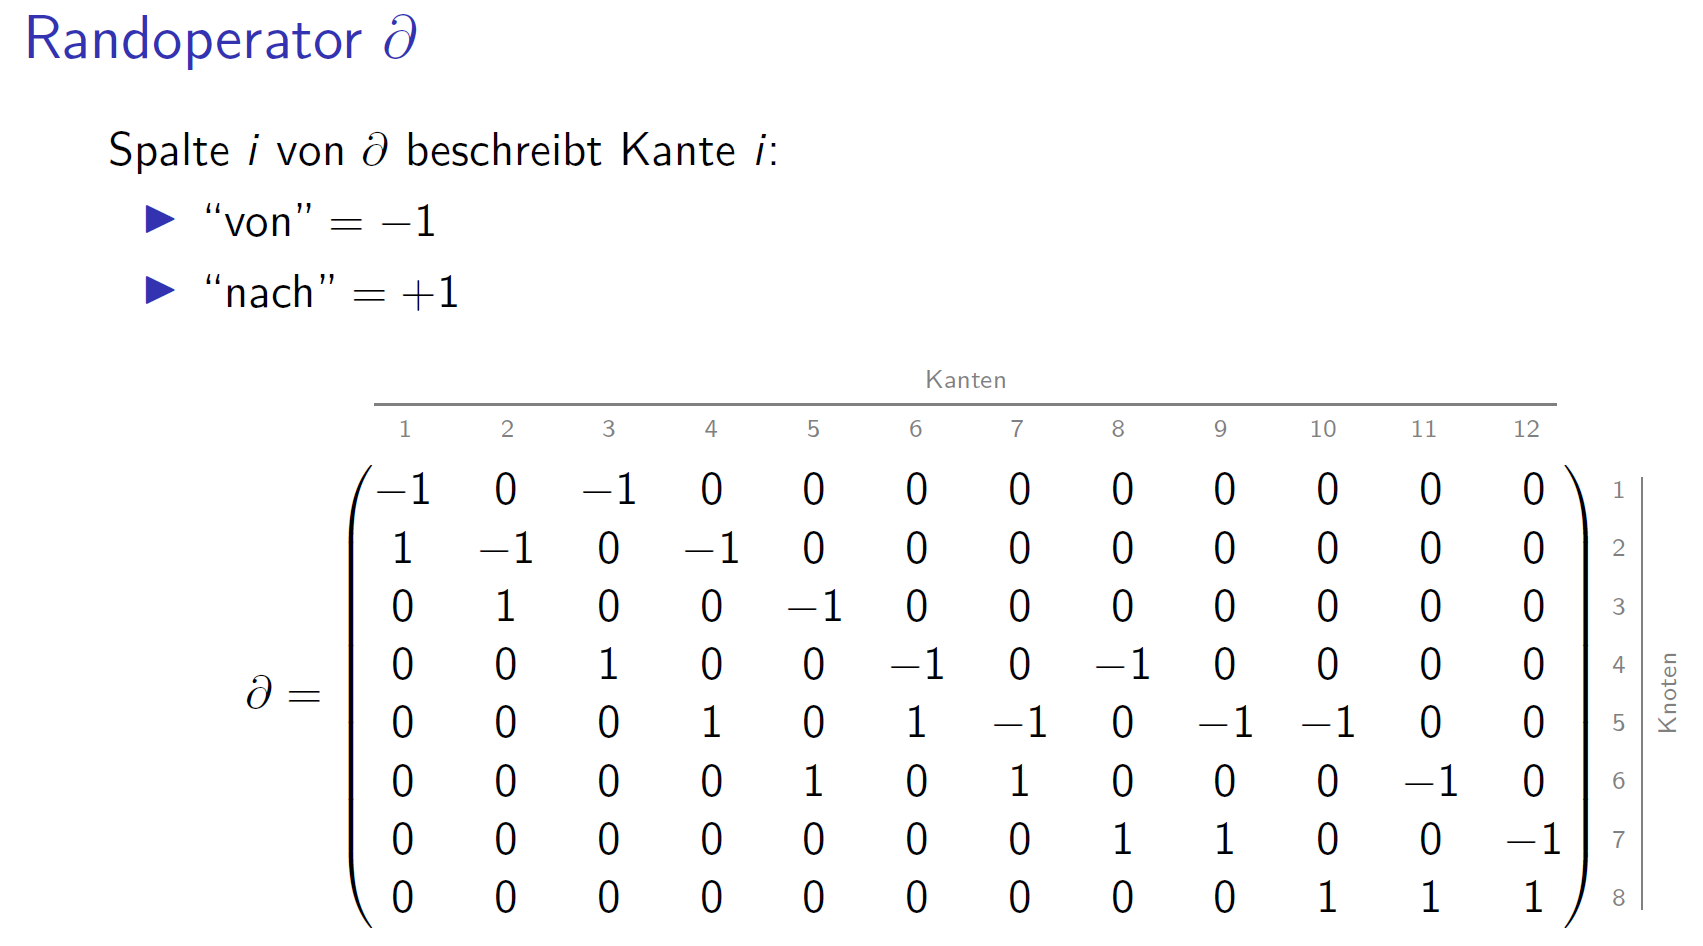
\includegraphics[width=0.8\linewidth]{Bilder/widerstand2} \\ 
		   
		   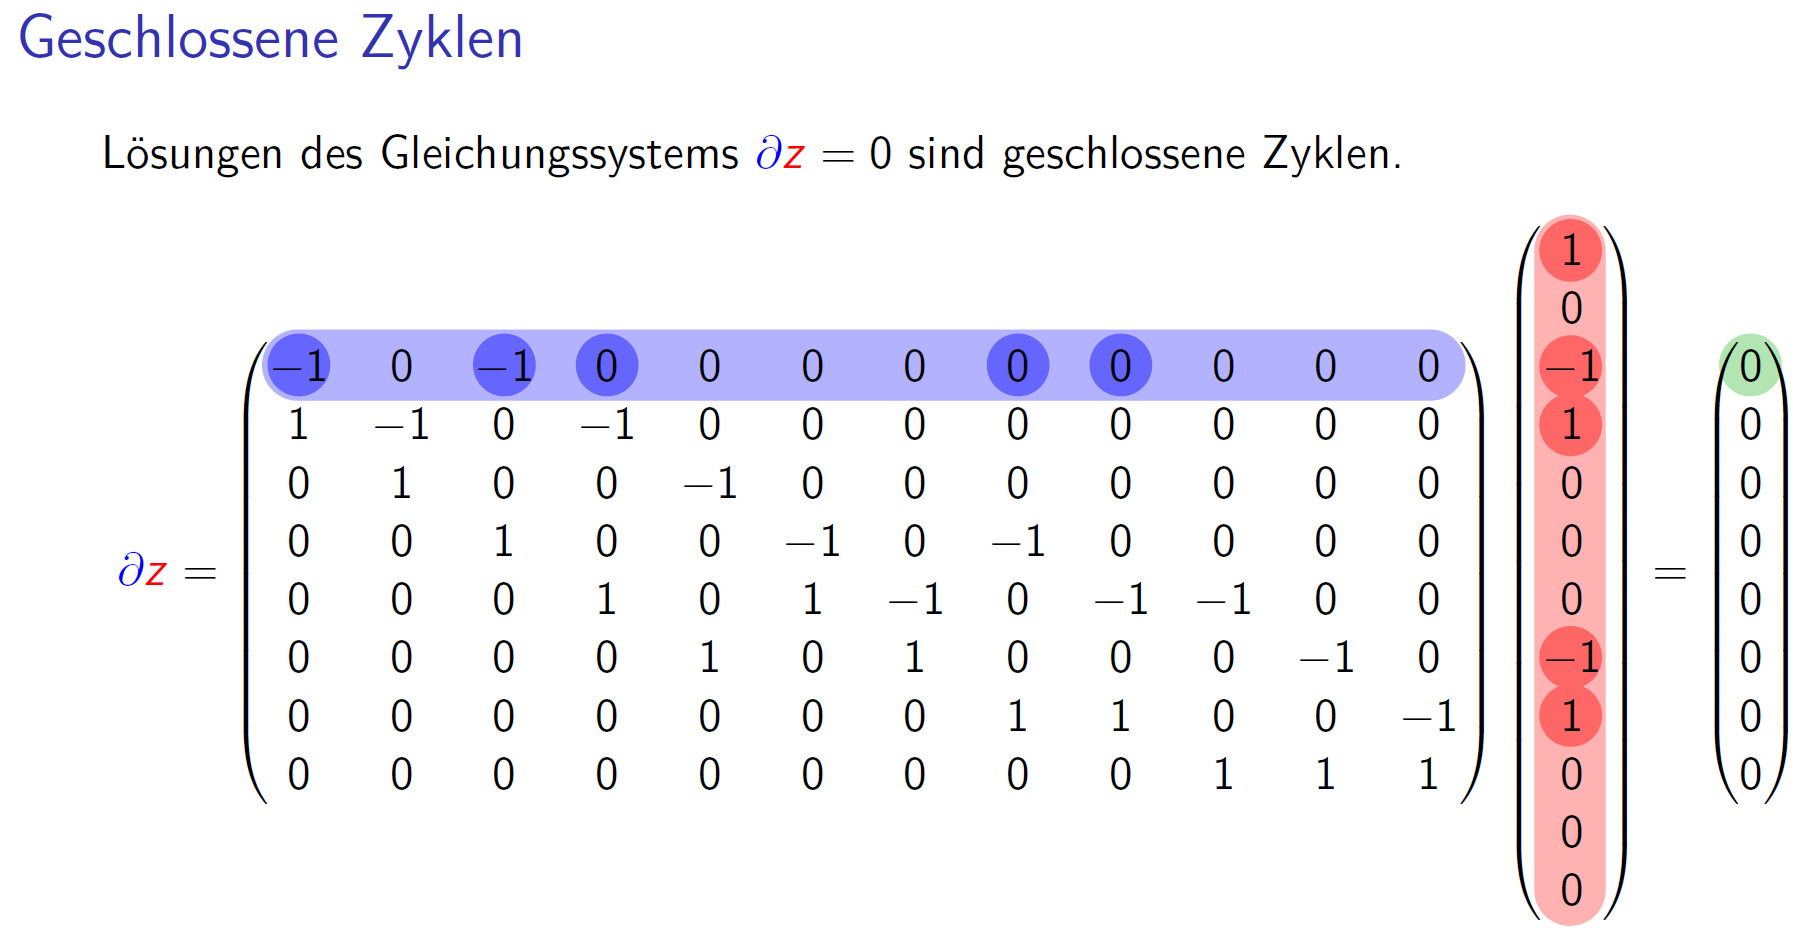
\includegraphics[width=0.8\linewidth]{Bilder/widerstand3} \\ 
		   
		   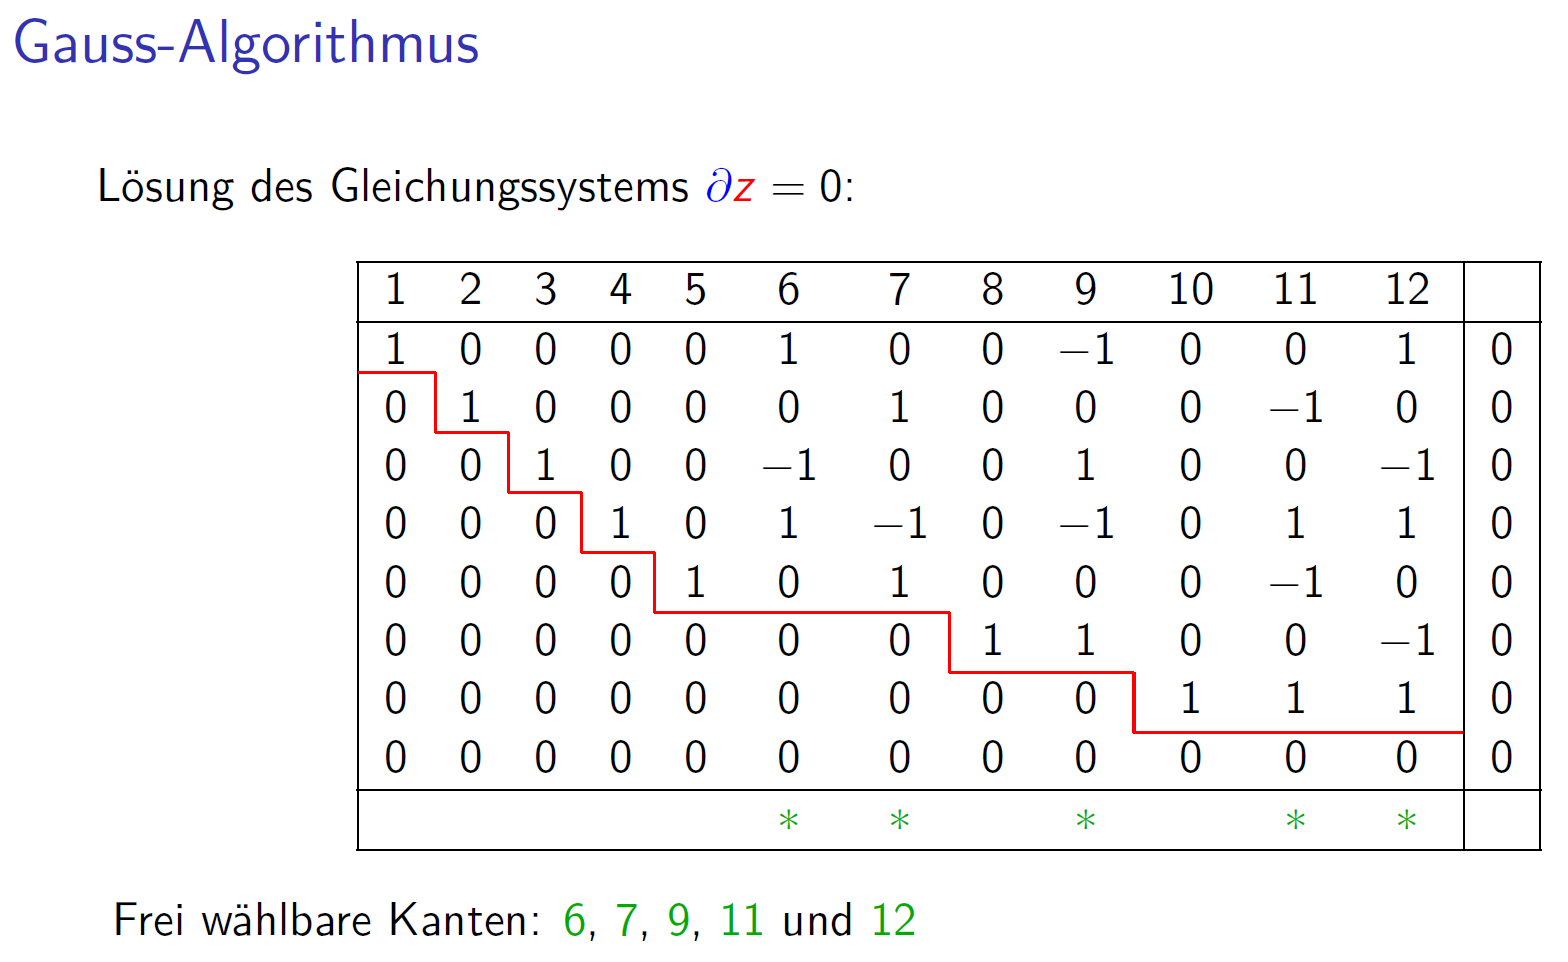
\includegraphics[width=0.8\linewidth]{Bilder/widerstand4} \\ 
		   
		   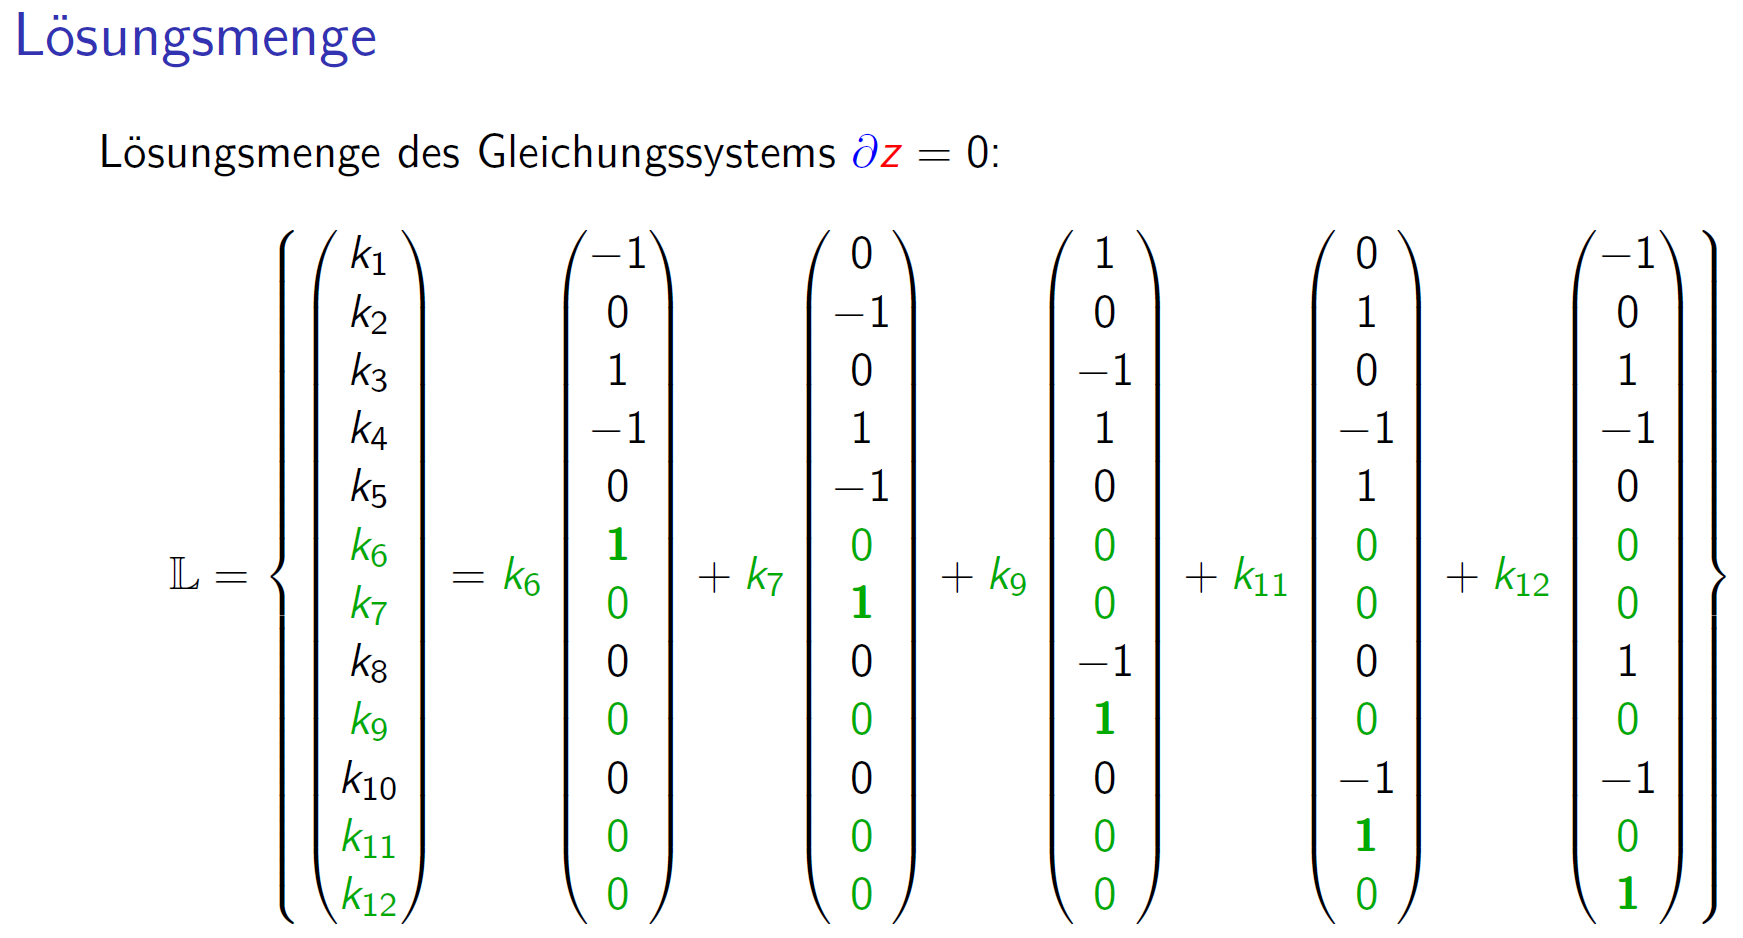
\includegraphics[width=0.8\linewidth]{Bilder/widerstand5} \\ 
		 